\section{The Progressive Second Price Auction}

A 'classic' second price auction is one in which a single, indivisible item is offered for sale. The winner is the bidder who bids the highest amount for the item, but the price they pay is not the price they bid, it's the price bid by the second-highest bidder.

This sounds like a strange concept, since it might not yield maximal profit, but it's actually how many auctions work. For example, the typical English auction, in which bidders call out progressively higher bids, is a second price auction. Two bidders will bid against each other, each raising the price in small increments until eventually one drops out. The other then wins the auction, but the price they pay has been determined by the bidder who withdrew from the bidding, not by their own evaluation of the item being sold.

Second price auctions have the very desirable property that they converge on a Nash equilibrium, meaning that no single bidder can improve their 'utility' by changing their bid. They also have the property that the optimal strategy for any bidder is to bid their true estimation of the value of the item being sold. This makes them the mechanism of choice for allocating resources in many social or market situations, where maximising profit is not the prime consideration.\footnote{While the English auction may not maximise profit for {\it rational} bidders, people often get carried away by the moment, and bid beyond their true valuation. Human psychology plays a large part in designing real-world auctions!}, rather the goal is to achieve a socially-acceptable distribution of resources.

The Progressive Second Price Auction (PSP)\cite{PSP} is an extension of the second price auction for single goods, specifically designed for allocating continuously divisible goods such as network bandwidth. This makes it suitable to form the core of a system that satisfies the requirements outlined earlier. The auction proceeds as follows:

\begin{enumerate}
\item[1)] The network offers a quantity {\bf Q} of bandwidth on a given network link.
\item[2)] Bidders have a given budget, not necessarily the same among bidders.
\item[3)] Bidders specify their bids in the form of a (quantity,unit-price) pair, (${\bf q_i}$,${\bf p_i}$).
\item[4)] The PSP algorithm calculates the allocation and total cost for each bidder, (${\bf a_i}$,${\bf c_i}$). The calculation is explained below.
\item[5)] PSP sends all allocations and costs to all bidders.
\item[6)] Bidders revise their bids if they aren't satisfied, and resubmit them.
\item[7)] Steps 3-6 are repeated until convergence.
\end{enumerate}

As shown in \cite{PSP}, convergence of the auction is guaranteed if players are rational. Rationality means, in essence, that they are willing to pay a higher unit-price to increase a small allocation than to increase a large one. In other words, the more they have, the less they are willing to pay to get even more. This is simply the market law of 'diminishing marginal returns'.

The PSP algorithm itself calculates allocations first, then the total cost per bidder. The allocations are calculated as follows:

\begin{enumerate}
\item[1)] Bidders are ranked in decreasing order of the unit-price they have bid.
\item[2)] The bidder with the highest unit-price gets his/her allocation first. If there is sufficient bandwidth for them to get the full quantity they requested, the request is granted in full. Otherwise, they get the remaining bandwidth, however much it is.
\item[3)] If there is any remaining bandwidth, step 2 is repeated for the next-highest bidder.
\end{enumerate}

This process is illustrated in figure~\ref{fig:allocation}

\begin{figure}[h]
 \centering
   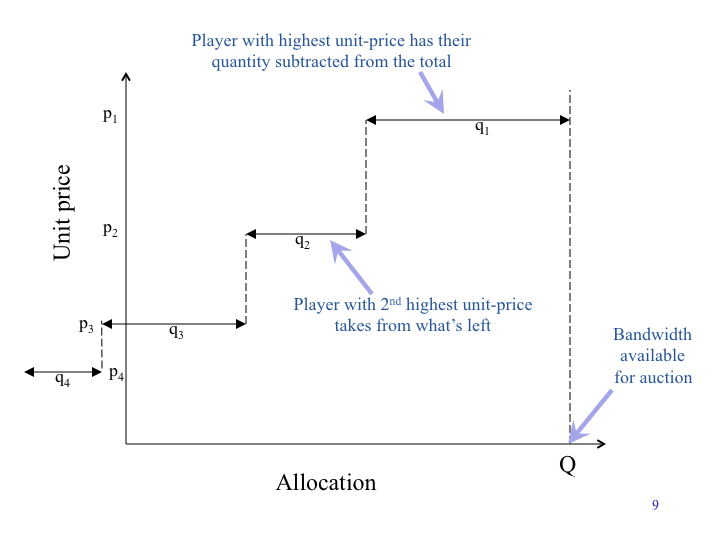
\includegraphics[width=0.8\textwidth]{allocation}
       \caption{The allocation procedure. The highest unit-price bidder is fully served, the second-highest is served from what's left, and so on. Bidders who bid too low are allocated zero bandwidth if it is all given to higher bidders.}
 \label{fig:allocation}
\end{figure}

The cost charged to a bidder is based on the 'exclusion compensation' principle, which extends the second-price principle. The fact that a given bidder {\it i} has bid may mean that other bidders are not granted the same allocation they would have if bidder {\it i} were not participating. Bidder {\it i} therefore pays for the amount by which they inconvenience those other bidders. I.e. for all bidders other than {\it i} who receive an allocation when {\it i} doesn't participate, the change in their allocation with bidder {\it i} participating is multiplied by the unit-price they were willing to pay, and the sum is the cost charged to bidder {\it i}.

Figure~\ref{fig:cost} illustrates this.

\begin{figure}[h]
 \centering
   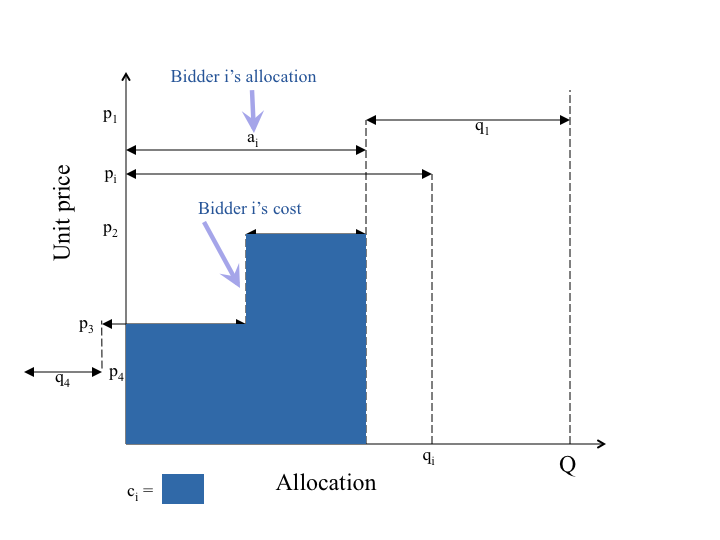
\includegraphics[width=0.8\textwidth]{cost}
       \caption{Calculating the cost for a new bid from bidder {\it i}. Bidder {\it i}'s allocation means bidders 2 and 3 lose their allocations, so their allocation is multiplied by their unit price, summed, and charged to bidder {\it i}.}
 \label{fig:cost}
\end{figure}

Also shown in \cite{PSP} are results from simulations with several tens of bidders all bidding on a single network link. The addition of a small 'reserve price' per unit bandwidth helps to ensure convergence in a short timescale by avoiding bids that change only in the lower decimal places, and still maintains the property of convergence on an \textepsilon -Nash equilibrium.